% % % % % % % % % % % % % % % % 
\section{Proposed Framework for an Ideal MRI Simulation System}
\label{chapterlabel4sec3}

This section focuses on introducing a generalised framework for an ideal \ac{mri} simulator to serve as a guideline for the \ac{mri} simulation community.
It is my belief that the proposed structure will aid in overcoming major limitations found throughout available simulators today and will also set the stage for my future work in my PhD project.
%Moreover, this framework can be used by the \ac{mri} simulation community as a unifying guideline.
This section gives an overview of the framework's components, while focusing on the simulation computational kernel.

\hfill

\large \textbf{Overview of framework} \normalsize

The proposed framework is summarised in Figure~\ref{fig:globalFramework} and it consists of the following 6 components:

\hfill

\textbf{Solver.} At the heart of this framework is the \textbf{Bloch Equation Solver}, which independently solves the Bloch equation for each spin in the input object.
The \textbf{solver} is a highly parallelizable component of the framework which can run either on a \ac{gpu} architecture.
The solver requires the following inputs:
\begin{itemize}
    \item \textbf{Sample Information}, such as:
    \textit{tissue specific parameters} (the nature of the nuclei, proton density, relaxation times and chemical shift), 
    \textit{geometry of the sample} (spin coordinates, resolution, total number of spins), and 
    \textit{motion trace} (translation and rotation values for each time point of the sequence).
    
    \item \textbf{Pulse Sequence Information}, such as:
    % \textit{Sequence Specific timings} (number of pulses in a multi-pulse sequence, repetition times and echo times),
    \textit{Radiofrequency Pulses} (amplitude and phase, duration, shape and timing), 
    \textit{Gradients} (shape, duration, timing) and
    \textit{Readout} (timing of each readout point).
    
    \item \textbf{Scanner Hardware Information}, such as:
    \textit{Main Magnet} (field strength, inhomogeneities in the main magnetic field),
    \textit{Gradient Limits} (maximum amplitude, slew rate) and
    \textit{Receiving/Transmitting Coils} (inhomogeneities in the coils, spatial sensitivity maps). 
\end{itemize}

\hfill

\textbf{Controllers.} The inputs described above are ubiquitous to any type of \ac{mri} simulation protocol.
However, my \textbf{Bloch equation solver} expects them in a certain format.
To overcome this limitation and to make my framework easily extensible, customisable and user friendly, I propose the existence of \textbf{Controllers}.
These are software wrappers which will translate user specific inputs into solver inputs.
With their help, the user can easily decide the complexity of the \ac{mri} simulation by choosing to include or exclude different sample specific, pulse sequence specific or hardware specific parameters.

\hfill

\textbf{Inputs.} The inputs to these controllers come in a variety of forms. 
For the sample object, the user can decide to either use a NIFTI phantom such as the \textit{BrainWeb digital brain phantom} \cite{Kwan1997}, or to create their own parameter maps consisting of the proton density, relaxation times and others.
If any of the required parameters are missing, a message will instruct the user about this error, while optional parameters will be omitted or set to some default values.

\hfill

For the pulse sequence, the user can decide to create their own sequence file consisting of timings ($T_R$, $T_E$), RF pulses ($N_{pulses}$, amplitude and phase), gradients (maximum amplitude, slew rate, shape) and readout timings, or they can use a scanner specific pulse sequence file.
%also choose to experiment with already created classic sequence such as gradient echo, echo planar imaging, etc, and only play with the
Finally, for the hardware configuration inputs, the user can choose to set the field strength ($B_0$) and the hardware limits for their simulation (maximum gradient amplitude, slew rate).
Additionally, for more complex scenarios, users can choose to include multi- transmit or receive coils with separate sensitivity maps or inhomogeneities in the coils.

\hfill

\textbf{GUIs. } Our framework also contains a set of \textbf{graphical user interfaces (GUIs)} which aid the end user in either rapidly prototyping new ideas or creating complex scenarios for \ac{mri} simulations.
Three GUIs are proposed: 
the \textit{Object GUI} for creating the input object and the motion trace,
the \textit{Pulse Sequence GUI} for creating the \ac{mri} pulse sequence and 
the \textit{Hardware Configuration GUI} for the hardware coil configuration.
The outputs from these GUIs become \textbf{inputs} for the software wrappers.

\hfill

\textbf{Reconstruction. } Having all of these in place, the \textbf{Bloch equation solver} will produce a set of signals corresponding to each coil used in the simulation.
These signals will be fed into a \textbf{reconstruction} block which, based on the type of readout used, can perform both Cartesian and non-Cartesian reconstructions.

\hfill

\textbf{Output. } The output of my proposed generalised framework is a set of reconstructed images and, if the option is enabled, the $x,y,z$ components of the magnetisation vector.
We have chosen to include the latter because in my experience with simulating \ac{mri} sequences, I have found it to be very useful to have this extra piece of information available to you.

\hfill

\large \textbf{GPU-Based Parallel Approach to the Bloch Equation Solver} \normalsize

The computational kernel of the \ac{mri} simulator will be based on the solutions of the Bloch equations at every time point in the pulse sequence and for every isochromat in the input object. 
These solutions will provide a temporal evolution of each isochromat's magnetisation vector under the effect of various \ac{rf} pulses, magnetic field gradients and inhomogeneities in the main magnetic field.

\hfill

Mathematically, the vector expression for the Bloch equation is:

\begin{flalign*}
    \frac{\vec{M}}{dt} &= \gamma \big( \vec{M} \times \vec{B}_{eff} \big) - 
    \begin{bmatrix}
    M_x / T_2 \\
    M_y / T_2 \\
    (M_z - \rho M_0) / T_1
    \end{bmatrix}
\end{flalign*}
where
\begin{flalign*}
    \vec{B}_{eff}(\vec{r},t) &= (xG_x(t) + yG_y(t)+ zG_z(t))\hat{z} + \Delta B (\vec{r}, t) \hat{z} + \vec{B}_{1x}(\vec{r},t) + \vec{B}_{1y}(\vec{r},t) 
\end{flalign*}
is the effective magnetic field experienced by the isochromat on position $\vec{r}$ and at time t,
$G_x, G_y $ and $G_z $ are the imaging gradients,
$\vec{B}_1$ is the applied RF pulse and 
$\Delta B$ accounts for off-resonance effects.

\hfill

The evolution of the magnetisation vector will be calculated by the computational kernel for every time-step $\Delta t$ in the pulse sequence using scaling and rotation matrices:
\begin{flalign*}
    \vec{M} (\vec{r}, t+\Delta t) &= (1-E_1) \vec{M}(t=0) + D \, \,  R_{eff} \, \,  \vec{M}(\vec{r},t)
\end{flalign*}
where $E_1 = e^{-\Delta t/T_1}$, 
$E_2 = e^{-\Delta t/T_2}$,
$\vec{M}(t=0)$ is the magnetisation vector at the beginning of the sequence, D is the diagonal matrix:
\begin{flalign*}
    D  & = \left[
    \begin{array}{c c c}
          E_2 &     0      &     0 \\
          0      & E_2 &     0 \\
          0      &     0      & E_1
    \end{array}
    \right]
\end{flalign*}
and $R_{eff} = R_{z}(\phi) R_{y}(-\beta) R_{x}(\alpha) R_{y}(\beta) R_{z}(-\phi)$ is the rotation matrix about the axis of the $\vec{B}_{eff}$ field.
Here, the $\vec{B}_{eff}$ field can have any orientation in the 3D space as it is characterised by the three $\alpha$, $\beta$ and $\phi$ angles.

\hfill

The simulation computational kernel will execute these matrix operations for every required time point in the sequence and for every isochromat in the object.
Due to its parallelisable nature, the simulation allows for groups of isochromats to be dealt with independently by the available stream processors.
The anatomical model will therefore be divided into smaller groups, based on the available resources of the \ac{gpu} card, and the computational kernel will be called for each of them.
The global memory of the \ac{gpu} will be populated with information about the pulse sequence, such that all available streaming processors can access it.
The shared memory of the stream processors will be populated with the components of the magnetisation vectors of each isochromat for every readout point.

\hfill

At the end of every kernel call these values will be transferred back to the \ac{cpu} and they will be summed over the previously computed signals.
The final complex signal $S(t)$ will be available when the entire simulation is done.
Finally, thermal noise will be added to the complex-valued signal.

\hfill

The proposed \ac{gpu}-based Bloch equation solver will be used to simulate advanced \ac{mri} sequences.
To allow for motion simulations, the spatial coordinates of the isochromats will be updated at every calculated time step of the pulse sequence.
Simple motion models that can be described analytically will be pre-computed on the \ac{cpu} and then stored in the \ac{gpu} global memory.
More complex motion models are also feasible, although they might increase the required GPU memory space.
In my future work, I am to investigate these further and come up with the best solutions for the remaining time of my PhD.

% Finally, it is my belief that this generalised framework can serve as a guideline for the \ac{mri} simulation community.
% This is because it both provides a seamless interface between many required \ac{mri} modules and
% it encourages the community to allow for integration of other open-source \ac{mri} units.
% For this reason, I also believe that it is important to develop this framework by using only open-source programming languages and packages.

\begin{figure}[ht]
    \centering
    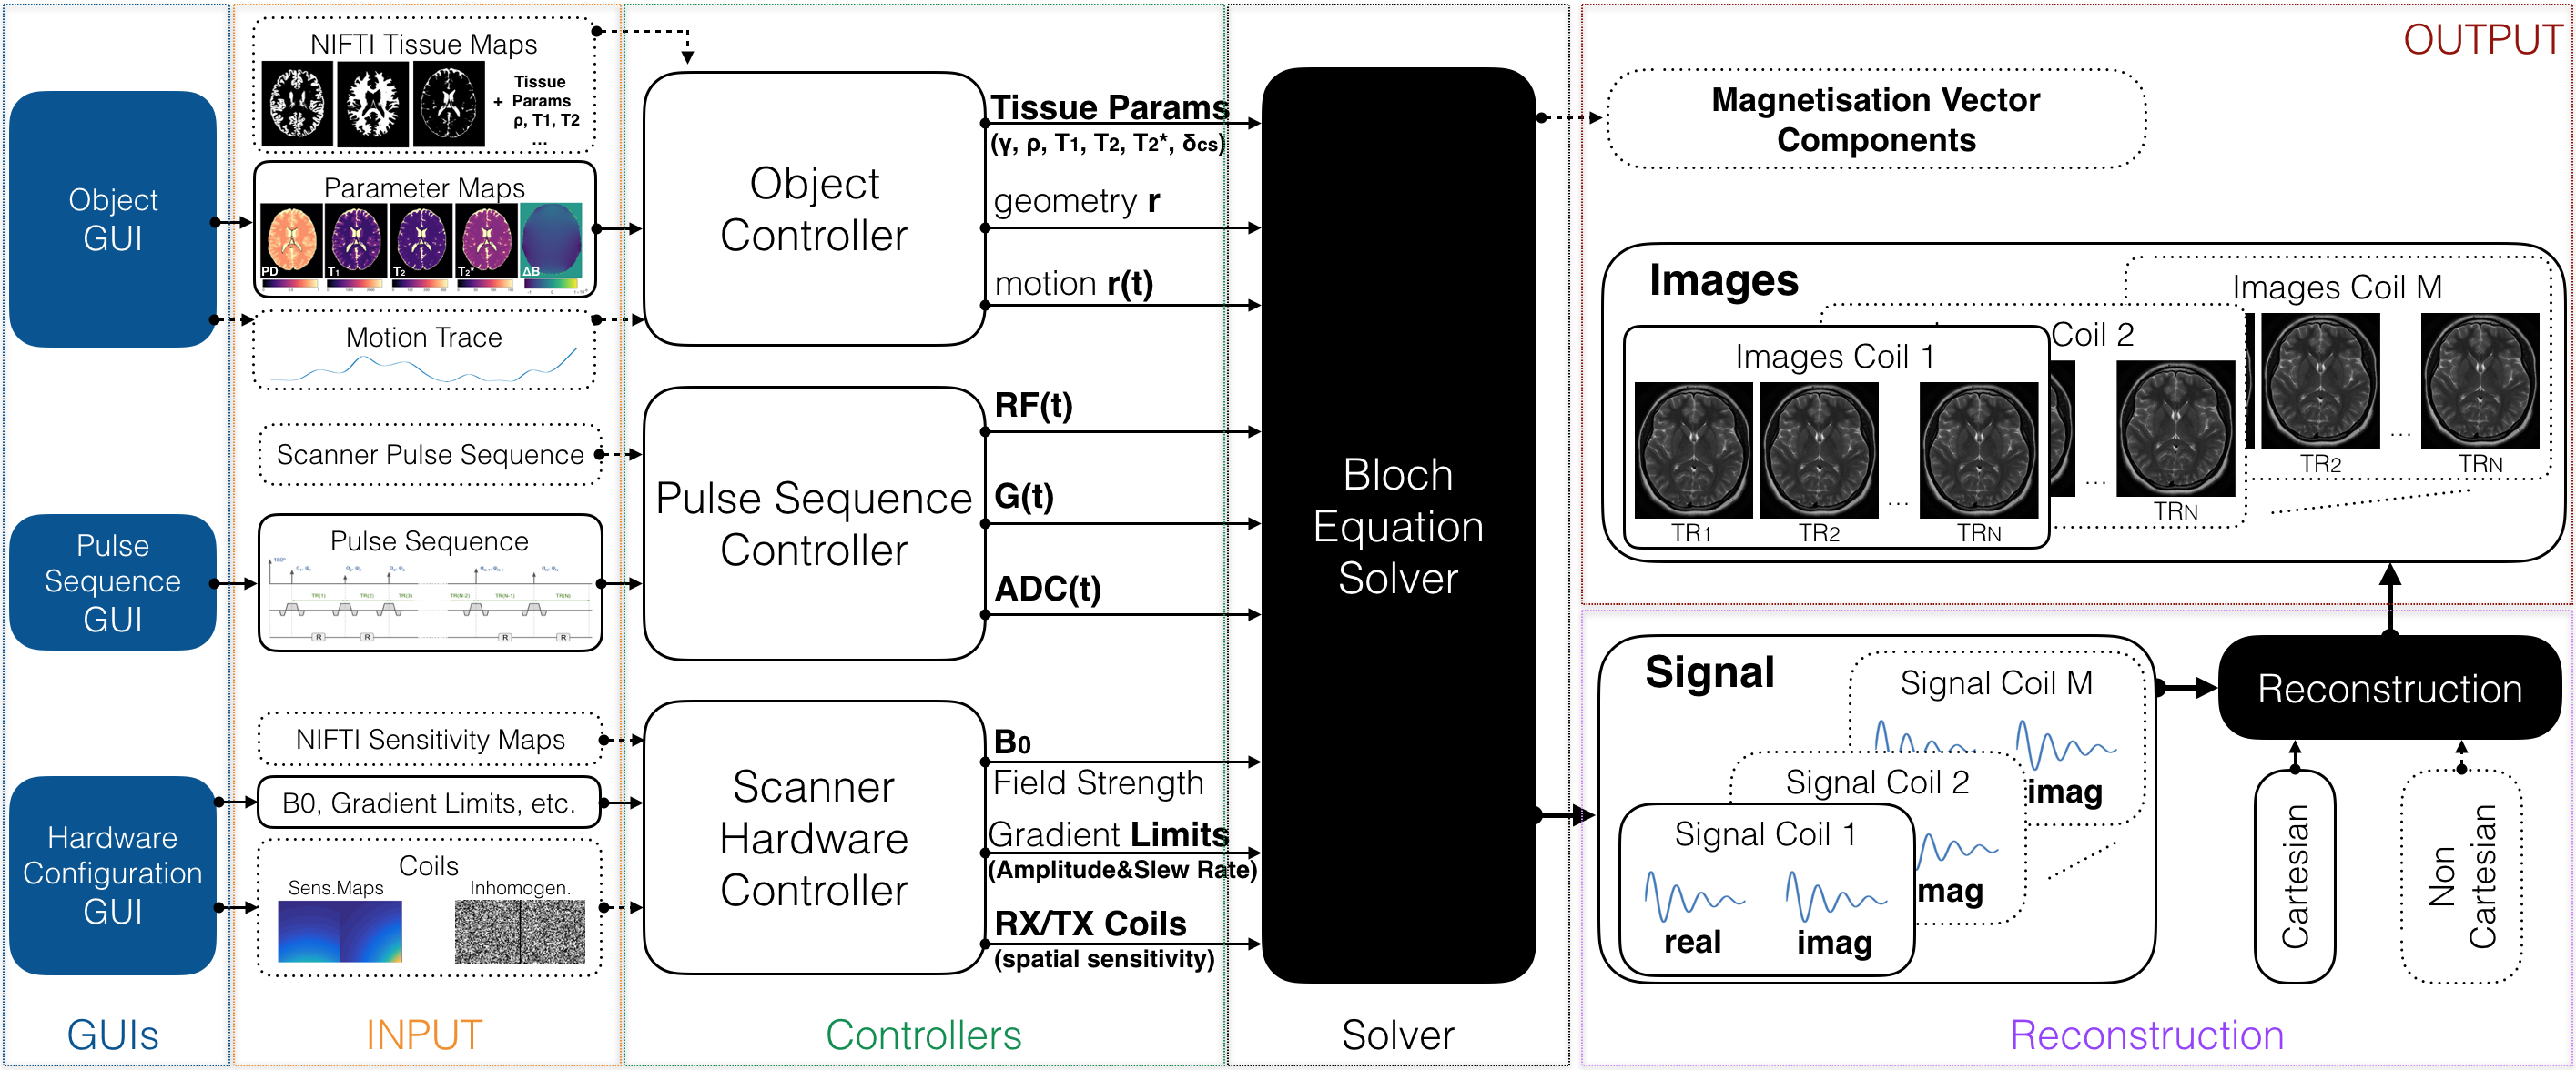
\includegraphics[angle=90,width=0.7\textwidth, keepaspectratio]{images/mri/globalFramework}
    \caption{Generalised framework for an ideal Magnetic Resonance Imaging simulator}
    \label{fig:globalFramework}
\end{figure}